% Lecture 15, Fig. 1: cross-section through a (normal) fault.
\documentclass[tikz,border=6pt]{standalone}
\usepackage{mathpazo}
\usetikzlibrary{arrows.meta}
\begin{document}
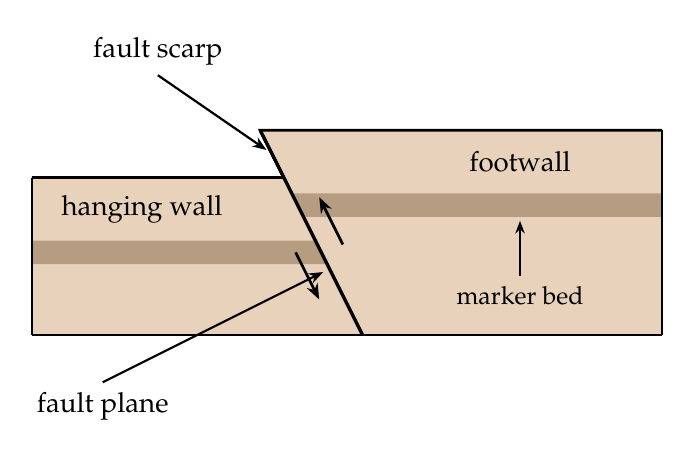
\begin{tikzpicture}[line width=0.8pt]
  \colorlet{rock}{brown!35!white}
  \colorlet{bed}{brown!70!black!60}
  % fault: from (4.2,0) at depth up to the surface at (2.85,2.7) (dips to the left)
  % hanging wall (left, above the fault plane, moved down); footwall (right, moved up)
  \fill[rock] (0,0) -- (4.2,0) -- (3.2,2.0) -- (0,2.0) -- cycle;
  \fill[rock] (4.2,0) -- (8,0) -- (8,2.6) -- (2.9,2.6) -- cycle;
  % a marker bed, offset across the fault
  \fill[bed] (0,0.9) -- (3.75,0.9) -- (3.6,1.2) -- (0,1.2) -- cycle;
  \fill[bed] (3.45,1.5) -- (8,1.5) -- (8,1.8) -- (3.3,1.8) -- cycle;
  % outlines: ground surface, scarp, fault
  \draw[line width=1pt] (0,2.0) -- (3.2,2.0) -- (2.9,2.6) -- (8,2.6);
  \draw[line width=1.2pt] (4.2,0) -- (2.9,2.6);
  \draw (0,0) -- (8,0) (0,0) -- (0,2.0) (8,0) -- (8,2.6);
  % relative motion
  \draw[-{Stealth[length=2mm]},line width=1pt] (3.35,1.05) -- (3.65,0.45);
  \draw[-{Stealth[length=2mm]},line width=1pt] (3.95,1.15) -- (3.65,1.75);
  % labels
  \node at (1.4,1.6) {hanging wall};
  \node at (6.2,2.2) {footwall};
  \draw[-{Stealth[length=1.8mm]}] (0.9,-0.6) node[below] {fault plane} -- (3.7,0.8);
  \draw[-{Stealth[length=1.8mm]}] (1.6,3.3) node[above] {fault scarp} -- (2.98,2.35);
  \node[font=\small] at (6.2,0.5) {marker bed};
  \draw[-{Stealth[length=1.6mm]}] (6.2,0.75) -- (6.2,1.45);
\end{tikzpicture}
\end{document}
